\documentclass[a4paper]{report}

\usepackage[dvips]{graphicx}

% This command makes sure we have reasonable margins.
\usepackage[]{fullpage}

%\usepackage{times}

% This statement puts a one-line spacing between two adjacent paragraphs
\setlength\parskip{\medskipamount}
% This statement cancels the indentation of the paragraph's first line
\setlength\parindent{0pt}

\begin{document}
\chapter{Modulo Circles}
\section{Modulo Graphs}

Given a natural number $ n $, we will look at the mapping
$ f(i) = 2i ~ (mod ~ n) $ for $ 0 \leq i \leq n-1 $. Furthermore, we
will draw a directed graph whose nodes are the numbers in that range.

Figure \ref{fig:graph-12-1} shows a sample graph for $ i = 12 $ :

\begin{figure}[ht]
\includegraphics{graph-12.eps}

\caption{\label{fig:graph-12-1} Modulo Graph for $ n = 12 $}
\end{figure}

\section{Modulo Graphs of Whole Powers of 2}

\begin{figure}[ht]
\begin{tabular}{ccc}
% The [scale=0.75] part resizes the image by 3/4
\includegraphics[scale=0.75]{graph-2.eps} &
\includegraphics[scale=0.75]{graph-4.eps} &
\includegraphics[scale=0.75]{graph-8.eps} \\
Modulo Graph for 2 &
Modulo Graph for 4 &
Modulo Graph for 8

\end{tabular}
\caption{Modulo Graphs of Powers of 2}
\label{fig:graphs-of-powers-of-2}
\end{figure}

As can be seen in Figure \ref{fig:graphs-of-powers-of-2} ~for whole powers
of 2,  the modulo graph is a binary tree, for which the fathers of $ i $ are
$ i/2 $ and $ i/2 + n/2 $. The root of the tree is $ n/2 $ which leads to 0.

Proving this is relatively trivial, so I won't go into there.

\section{Even Numbers}

Let's take the modulo graph of 12 and compare it with the modulo graph of
3 (the incenitive for this is that $ 12 = 3 \cdot 2^{2} $). One can find
both of them in Figure \ref{fig:graphs-of-3-and-12}.

\begin{figure}[ht]
\begin{tabular}{c||c}
\includegraphics[scale=0.75]{graph-3.eps} &
\includegraphics[scale=0.75]{graph-12.eps} \\
Modulo Graph for 3 &
Modulo Graph for 12
\end{tabular}
\caption{Graphs of 3 and 12}
\label{fig:graphs-of-3-and-12}
\end{figure}

One can notice that the modulo graph of 12 is in fact the modulo graph
of 3 multiplied by 4, while every vertex of this graph serves as the "zero"
for a 4-like tree. This is in fact the general case for $ n' \cdot 2^{e} $,
and again it can be easily proven.

\section{Prime Numbers}

% I decide to avoid using these macros
%\newcommand{\var}[1]{{\bf #1}}
%\newcommand{\myvar}{\var{a}}
Assume that $ a $ is a given modulo. In order to find the size of its
circle, one has to find what is the $ n $ so that $ a\cdot2^{n} $ modulo
the reminder gives $ a $.

We will first deal only with prime numbers (the circle's modulo will be
indicated with $ p $.

% Note that the ampersand sign (&) is a separator
% that separates the columns of the table. The entire table is
% centered around the middle cell in each row.
\begin{eqnarray*}
2^{n} \cdot a (mod ~ p) & = & a
\\
2^{n} \cdot a - p \cdot m & = & a  ~  \mbox{( So that m is maximal )}
\\
2^{n} \cdot a - a & = & p \cdot m
\\
2^{n} - 1 & = & \frac{p \cdot m}{a}
\\
2^{n} & = & \frac{p}{a} \cdot m + 1
\end{eqnarray*}

Since $ p $ is a prime number it is not divisable by $ a $ or by
one of its factors. Therefore, $ m $ is divisable by $ a $. (in accordance
with Fermat's Theorem) I will define a natural number $ m' = \frac{m}{a} $
and one can see that $ 2^{n} = p \cdot m' + 1 $.

$ n $ ought to be minimal, and that is the size of the circle. One can
see that when the dividing number is prime, there isn't any significance
for $ a $ and thus, the size of all the circles (beside that of 0) is
equal!

From this it can be seen that their number may be derived by the forumula
$ N_{circ}=\frac{p-1}{n}+1 $

\section{A product of several distinct prime numbers}

Let's assume $ n = p_{1} \cdot p_{2} $ . Such number has a circle of 0,
and circles for each of his factors, so that their numbers are multiplied
by the other factor. It also has several circles which are unique to it.
It can be easily deduced that the total length of these circles is
$ (p_{1} - 1)(p_{2} - 1) $. They are all of equal length, which can be determined
by passing a number that is not divisable by $ p_{1} $ or $ p_{2} $ through
it. 2 is a good choice for such a number.

The same paradigm can be induced to multiplications of more than two prime
factors.

\section{Powers of a prime number}

Let's mark the unique circle length of a number $ n $ by $ Sh(n) $.

In that case, the number of unique circles of $ p^{n} $ is
$ \frac{p^{n}(p-1)}{Sh(p^{n})} $. Let's prove that it is a constant, which
is dependant on $ p $ alone. It can be seen that in order to prove that,
one can prove that $ Sh(p^{n+1}) = p \cdot Sh(p^{n}) $.

Let's mark $ t = Sh(p^{n}) $ and $ t'=Sh(p^{n+1}) $. One has to prove that
$ t' = p \cdot t $.

It is known that $ 2^{t} (mod ~ p^{n}) = 1 $. Thus:

$ 2^{t} = a \cdot p^{n} + 1 $ (where $ a < p $ is a certain number)

What power of $ (a \cdot p^{n} + 1 ) $ will divide by $ p^{n+1} $ with
a modulo of 1? According to Newton's binomial, it will be:

\[
(a \cdot p^{n} + 1)^{m} = A_{m}p^{nm} + A_{m-1}p^{n(m-1)} + ... + A_{2}p^{2n} + A_{1}p^{n} + 1
\]

It can be seen that all the exponents up to and including $ p^{2n} $ are easily
divisable by $ p^{n+1} $. So we have to make sure $ A_{1}p^{n} $ is divisable
by $ p^{n+1} $. (since we already have the reminder of 1 in the last element)

According to the Newton's binomial formula $ A_{1} $ is equal to:

\[
A_{1} = m \cdot a \cdot p^{n}
\]

Because $ p $ is prime, it would divide by $ p^{n+1} $ only when $ m $ is equal
to $ p $. Thus, one has to raise everything to the power of $ p $ and thus,
according to the laws of exponentation $ t'=p \cdot t $. Q.E.D.

\section{Determining the unique circle length of a product}

$ Sh(q_{1} \cdot q_{2}) = lcm(Sh(q_{1}), Sh(q_{2})) $ assuming
that $ q_{1} $ and $ q_{2} $ are strangers. To prove that, one needs
to visualize that every time one multiplies by 2 and takes the reminder, there
is an advance on each one of the factors' circles. Thus, they will return
to the beginning only when the number of steps will divide by the circle
length of each one, fully.

This proves that the unique circle length of the product is divisable by the
lcm, but does not prove that it is equal to it. To prove the latter
conjectyre, one can rely on the fact that the field of the modulos of
the product is spanned by the modulo fields of the factors (assuming
they are indeed two stranger numbers). Thus, two respective given
modulos for each of the factors implies one unique modulo for the
product. Q.E.D.

\section{Acknowledgements}

The material in these pages is based on a lecture I attended by
Prof. Amos Ehrlich (http://www.tau.ac.il/~amos1/) of Tel-Aviv University.

The modulo graphs were rendered using GraphViz
(http://www.research.att.com/sw/tools/graphviz/)

\end{document}

